\documentclass{standalone}

\usepackage{tikz}
\usetikzlibrary{arrows.meta}

\begin{document}

\noindent
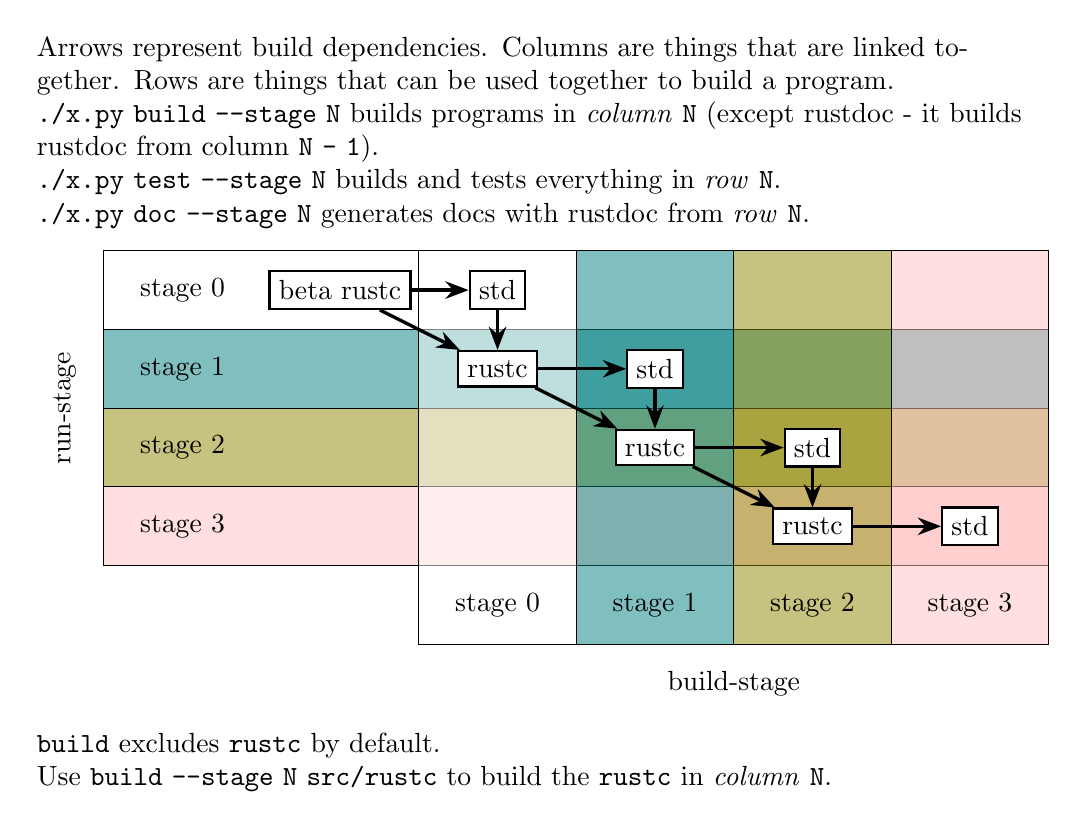
\begin{tikzpicture}

\node[text width=5in] at (2.5, 2) {
\noindent Arrows represent build dependencies.
Columns are things that are linked together.
Rows are things that can be used together to build a program.
\\

\noindent \verb|./x.py build --stage N| builds programs in \emph{column} \verb|N| (except rustdoc - it builds rustdoc from column \verb|N - 1|).\\
\noindent \verb|./x.py test --stage N| builds and tests everything in \emph{row} \verb|N|.\\
\noindent \verb|./x.py doc --stage N| generates docs with rustdoc from \emph{row} \verb|N|.\\
};

\draw[draw=black,fill=white,fill opacity=0.5] (-3, -0.5) rectangle ++(12, 1);
\draw[fill=teal,fill opacity=0.5] (-3, -1.5) rectangle ++(12, 1);
\draw[fill=olive,fill opacity=0.5] (-3, -2.5) rectangle ++(12, 1);
\draw[fill=pink,fill opacity=0.5] (-3, -3.5) rectangle ++(12, 1);

\draw[draw=black,fill=white,fill opacity=0.5] (1, 0.5) rectangle ++(2, -5);
\draw[fill=teal,fill opacity=0.5] (3, 0.5) rectangle ++(2, -5);
\draw[fill=olive,fill opacity=0.5] (5, 0.5) rectangle ++(2, -5);
\draw[fill=pink,fill opacity=0.5] (7, 0.5) rectangle ++(2, -5);

\node[rotate=90] at (-3.5, -1.5) {run-stage};

\node[] at (-2, 0) {stage 0};
\node[] at (-2, -1) {stage 1};
\node[] at (-2, -2) {stage 2};
\node[] at (-2, -3) {stage 3};

\node[] at (5, -5) {build-stage};

\node[] at (2, -4) {stage 0};
\node[] at (4, -4) {stage 1};
\node[] at (6, -4) {stage 2};
\node[] at (8, -4) {stage 3};

\begin{scope}[every node/.style={thick,draw,fill=white}]
	\node (s0r) at (0,0) {beta rustc};
	\node (s0s) at (2,0) {std};
	\node (s1r) at (2,-1) {rustc};
	\node (s1s) at (4,-1) {std};
	\node (s2r) at (4,-2) {rustc};
	\node (s2s) at (6,-2) {std};
	\node (s3r) at (6,-3) {rustc};
	\node (s3s) at (8,-3) {std};
\end{scope}

\begin{scope}[>={Stealth[black]}, every edge/.style={draw=black,very thick}]
	\path [->] (s0r) edge node {} (s0s);
	\path [->] (s0r) edge node {} (s1r);
	\path [->] (s0s) edge node {} (s1r);
	\path [->] (s1r) edge node {} (s1s);
	\path [->] (s1r) edge node {} (s2r);
	\path [->] (s1s) edge node {} (s2r);
	\path [->] (s2r) edge node {} (s2s);
	\path [->] (s2r) edge node {} (s3r);
	\path [->] (s2s) edge node {} (s3r);
	\path [->] (s3r) edge node {} (s3s);
\end{scope}

\node[text width=5in] at (2.5, -6) {
\noindent \verb|build| excludes \verb|rustc| by default.

Use \verb|build --stage N src/rustc| to build the \verb|rustc| in \emph{column}
\verb|N|.
};

\end{tikzpicture}

\end{document}
